

\subsection{Conformal Prediction}
%\sofi{highlight the difference between conformal and split, differenciation}

We briefly review the algorithm and guarantees for conformal prediction, and refer readers to~\cite{angelopoulos2021gentle} for a thorough introduction. In this paper CP refers to \textit{split conformal prediction} (we consider full conformal prediction out of scope, because its computationally complexity renders it nonviable for deep learning settings). The goal of conformal prediction is to produce a \textit{valid} prediction interval (Def.~\ref{def:validity}) for any underlying prediction model.
%
\begin{definition}[Validity]
Given a new data point $(x,y)$, where $y$ is the prediction target and $x$ is the covariates,  and a desired confidence $1-\alpha \in (0,1)$, the prediction interval $\Gamma^{1-\alpha}(x)$ is a subset of $\mathcal{Y}$ containing probable outputs given $x$. The region $\Gamma^{1-\alpha}$ is valid if
%
\begin{equation}\label{eq:coverage}
P (y \in \Gamma^{1-\alpha}(x)) \geq 1-\alpha
 \end{equation}
\label{def:validity}
\end{definition}
%
\vspace{-2em}
Let $\mathcal{D} = \{ (x^i, y^i)\}_{i=1}^n$ be a dataset whose data points $(x^i, y^i)$ are sampled from a distribution on $ \mathcal{X} \times \mathcal{Y}$.  Conformal prediction splits the dataset into a proper training set $\Dtrain$ and a calibration set $\Dcal$. A prediction model $\hat{f}: \mathcal{X} \rightarrow  \mathcal{Y}$ is trained on $\Dtrain$. We use a \textit{nonconformity score} function $A: \mathcal{X} \times  \mathcal{Y} \rightarrow \R_{\geq 0}$ to quantify how well a data sample from calibration \textit{conforms} to the training dataset. Typically, we choose a metric of disagreement between the prediction and the true label as the non-conformity score, such as the Euclidean distance: 
%
\begin{equation}
 A(x,y) \stackrel{\text{e.g.}}{=} d(y,\hat{f}(x)) \stackrel{\text{e.g.}}{=} 
\|y - \hat{f}(x)\|_2 
\label{def:non-c}
\end{equation}
%
Let $\gS = \{A(x^i, y^i)\}_{(x^i, y^i) \in \Dcal}$ denote the set of nonconformity scores of all samples in the calibration set $\Dcal$. %We define a quantile function for nonconformity scores $\gS$ as:
%
During inference time given a new data  $x^{n+1}$, the conformal prediction interval is constructed as in \Eqref{eq:region}, where $Q$ is the empirical quantile function. 
%
\begin{equation}
    \Gamma^{1-\alpha}(x^{n+1}):=  \{ y : A(x^{n+1}, y) \leq Q^{1-\alpha}(\gS \cup \{\infty\})\}  
    \label{eq:region}
\end{equation}
%
% \begin{equation}
%     Q(1-\alpha, \gS) := \text{inf} \{s^*: (\frac{1}{|\gS|} \sum_{s^i \in \gS} \mathbbm{1}_{s^i \leq s^*}) \geq 1-\alpha \}
%     \label{eq:quantile}
% \end{equation}
We say a sample is \textit{covered} if the true value lies in the prediction interval $y^{n+1} \in \Gamma^{1-\alpha}(x^{n+1})$ %and define \textit{coverage} as $P(y^{n+1} \in \Gamma(x^{n+1}))$. 
Conformal prediction is guaranteed to produce valid prediction intervals \citep{vovk2005algorithmic} if the calibration data and test data are exchangeable (in a dataset $\{(x^i, y^i)\}_{i=1}^n$ of size  $n$, any of its $n$! permutations are equally probable).


Conformal prediction has been extended to the online setting. More precisely, the algorithm observes $(x_1, y_1), (x_2, y_2), \ldots$ sequentially, and needs to construct a prediction set $ \Gamma^{1-\alpha}_t$ for $y_t$ at time step $t$. Without making any distributional assumptions on the data generation process, online CP algorithms achieve asymptotic guarantee as \Eqref{eq:aci_convergence}, where $\mathbbm{1}\{\cdot\}$ is the indicator function:
\vspace{-0.5em}
\begin{equation}
\lim_{T \to \infty} \frac{1}{T} \sum_{t=1}^T \mathbbm{1}\{ y_t \notin \Gamma^{1-\alpha}_t(x_t) \} = \alpha  \label{eq:aci_convergence}
\end{equation}

\vspace{-1em}
We refer readers to \cite{angelopoulos2024theoretical} for a summary of theoretical results in this setting.


\subsection{Switching Dynamical Systems for Modeling Time-series with Change Points}
\label{background:sds}
%Switching dynamics systems (SDS), or mixed dynamics systems, is a setting motivated by many real-world scenarios where a single time series model is insufficient to capture the complex and heterogeneous patterns in temporal data. 


\begin{figure}
    \centering
	%\subfloat{\scalebox{0.85}{\input{changepoints/figs/generative.tikz}}}
     \vspace{-2em}
    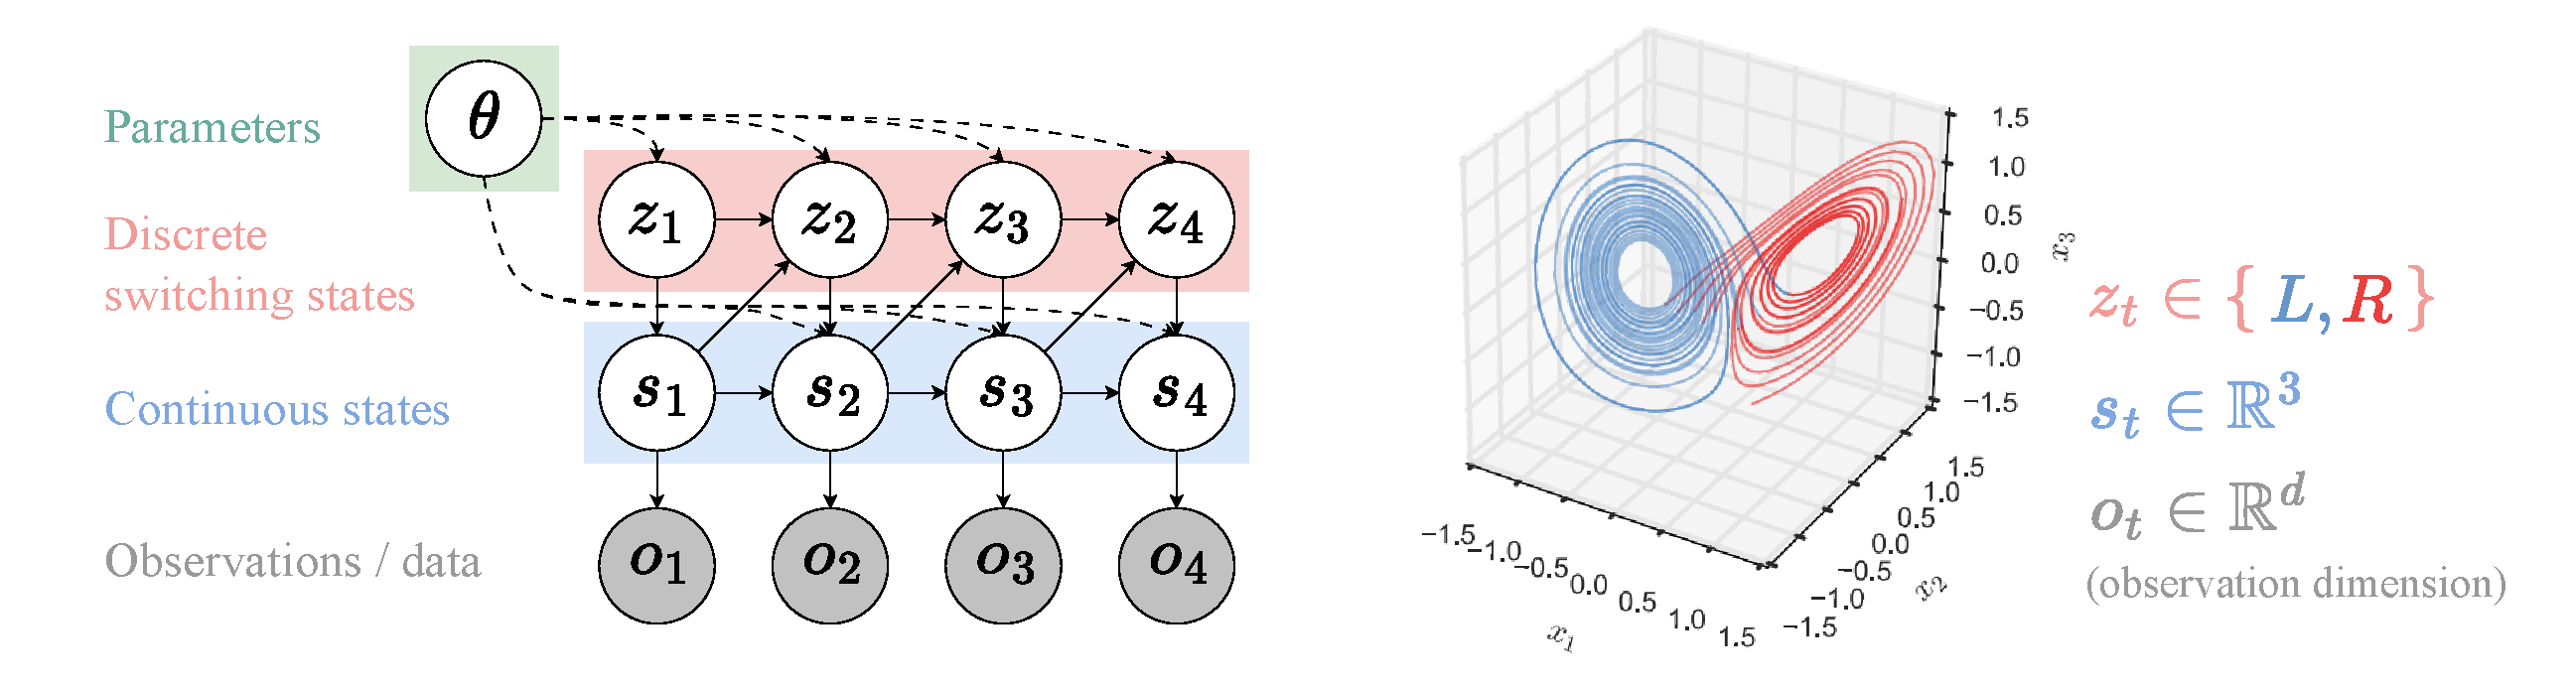
\includegraphics[width=\linewidth]{changepoints/figs/sds.pdf}   \vspace{-1em}
	\caption{(Left) Generative model of the SDS dynamics as in \Eqref{eq:sds}. Shaded circles represent observed  variables; hollow circles are latent variables. (Right) Example to illustrate notation. We show a Lorenz attractor, a canonical nonlinear dynamical system, approximated by a linear SDS \cite{linderman2023slds}.}
	\label{fig:sds_figure}
         \vspace{-1.5em}
\end{figure}

Switching dynamics systems (SDS), or mixed dynamics systems, provide a powerful framework for modeling time series with change points, where the underlying dynamics shift between distinct regimes. SDS assumes the system consists of a total of $K$ different base dynamics. It explicitly incorporates discrete switching \textit{states} to represent the abrupt shifts among base dynamics. We denote the discrete switching states at timestep $t$ as $z_t \in \mathcal{Z}$, $ \mathcal{Z} = \{1, \dots, K\} \subset \mathbb{Z}^+$, to index one of $K$ base dynamical systems, and represent the observed sequence as ${o_1, \ldots, o_T }$ or $o_{1:T}$ for conciseness. %Since continuous states $s_t$ are rarely discussed, we use \textit{state} to refer to discrete states $z_t$ if not otherwise indicated.

There have been many different variations and implementations of SDS.  Classic SDS have \textit{memory-less} state transitions, i.e. $p(z_t|z_{t-1})$ is parameterized by a stochastic transition matrix $\mathbf{A}\in \R ^{K \times K}$. 
This results in an “open loop” system and the state  duration follows a geometric distribution. Recent works have sought to fix this issue, for example by closing the loop using recurrent dependencies on $s_t$ \citep{linderman2016recurrent}, or modeling explicit durations \citep{ansari2021deep}. Our generative model is illustrated in figure \ref{fig:sds_figure}): for generality, we factor out any non-Markovian covariates to model parameters $\theta$. The joint distribution can be factorized as
\vspace{-1em}
\begin{equation} \label{eq:sds}    
\begin{split} 
& P(o_{1:T}, s_{1:T}, z_{1:T} ) =  \prod^T_{t=1} P(o_t | s_t) P(s_t| s_{t-1}, z_t, \theta) P(z_t| s_{t-1}, z_{t-1},\theta)
\end{split}
\end{equation}

\vspace{-1.5em}
where $p(s_1|z_1)p(z_1)$ is the initial state prior. The $K$ dynamical systems have continuous state transition $p(z_t|z_{t-1}, s_{t-1}, \theta)$, and the emission  $p(o_t| s_t)$ can be linear or nonlinear (e.g. parameterized by a neural network). Moreover, the SDS framework naturally supports forecasting both the next observation \(o_{t+1}\) via
$P(o_{t+1}\mid s_{t+1})$
and the next switching state \(z_{t+1}\) via
$P(z_{t+1}\mid s_t, z_t, \theta).$
